\documentclass[10pt]{article}
\usepackage{listings}
\usepackage{float}
\usepackage{graphicx}
\usepackage{fullpage}
\usepackage{caption}
\usepackage{subcaption}
\usepackage{amsmath}
\usepackage{hyperref}

%\renewcommand{\thesubsection}{\arabic{subsection}}
\renewcommand{\thesubsubsection}{\alph{subsubsection}}

\title{Pattern Recognition Practical 3}
\author{Group 24: \and Maikel Withagen (s1867733) \and Steven Bosch (s1861948)}
\date{\today}
\lstset{
frame=single, 
numbers=left, 
breaklines=true, 
language=Matlab,
basicstyle=\small, 
title=\lstname,
showstringspaces=false
}

\renewcommand{\thesection}{Assignment \arabic{section}}
\renewcommand{\thesubsection}{\arabic{subsection}}
\begin{document}

\maketitle

\section{Classification error, hit/false alarm rates, ROC curve, discriminability}
\subsection{}
Figure \ref{fig1.1} shows the ROC-curves we acquired using the code given in the listing for assignment 1.1 in the appendix. The figure shows that the higher the difference between the means of the two distributions is (i.e. the further away the distributions are from each other), the higher the number of hits is per number of false alarms. This suggests that classification goes better when distributions are further away from each other.

\begin{figure}[H]
 \centering
 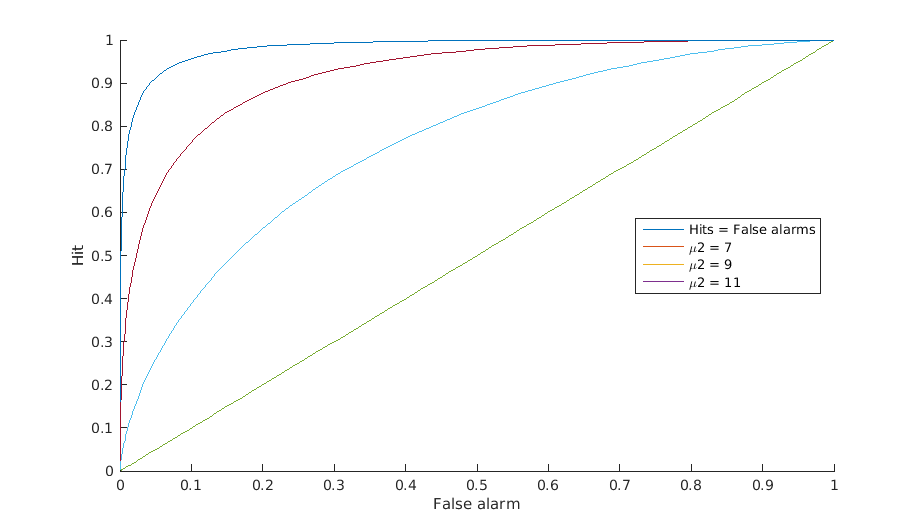
\includegraphics[width=\textwidth]{assign1_1.png}
 \caption{ROC-curves for $\mu_2={7, 9, 11}$ and the hits $=$ false alarms marker line.}
 \label{fig1.1}
\end{figure}

\subsection{}
\autoref{fig1.2} shows the point $(fa, h)$ of the two given binary vectors plotted in the figure from assignment 1.1. The listing for assignment 1.2 in the appendix gives the code used to compute this point and to compute the ROC-curve with the associated discriminability value $d'$. Trial and error yielded a ROC-curve with $d' \approx 1.5$ (this is an approximation, the exact value is a decimal value that is time-consuming to find by trial and error). We computed this using $\sigma_{1,2} = 1$, which yields $\mu_2-\mu_1 = 1.5$ for the found discriminability value. Note that the code in the listing gives $\sigma = 2$, which means $\mu_2-\mu_1 = 3$, since $d' = \frac{\mu_2-\mu_1}{\sigma}$.

\begin{figure}[H]
 \centering
 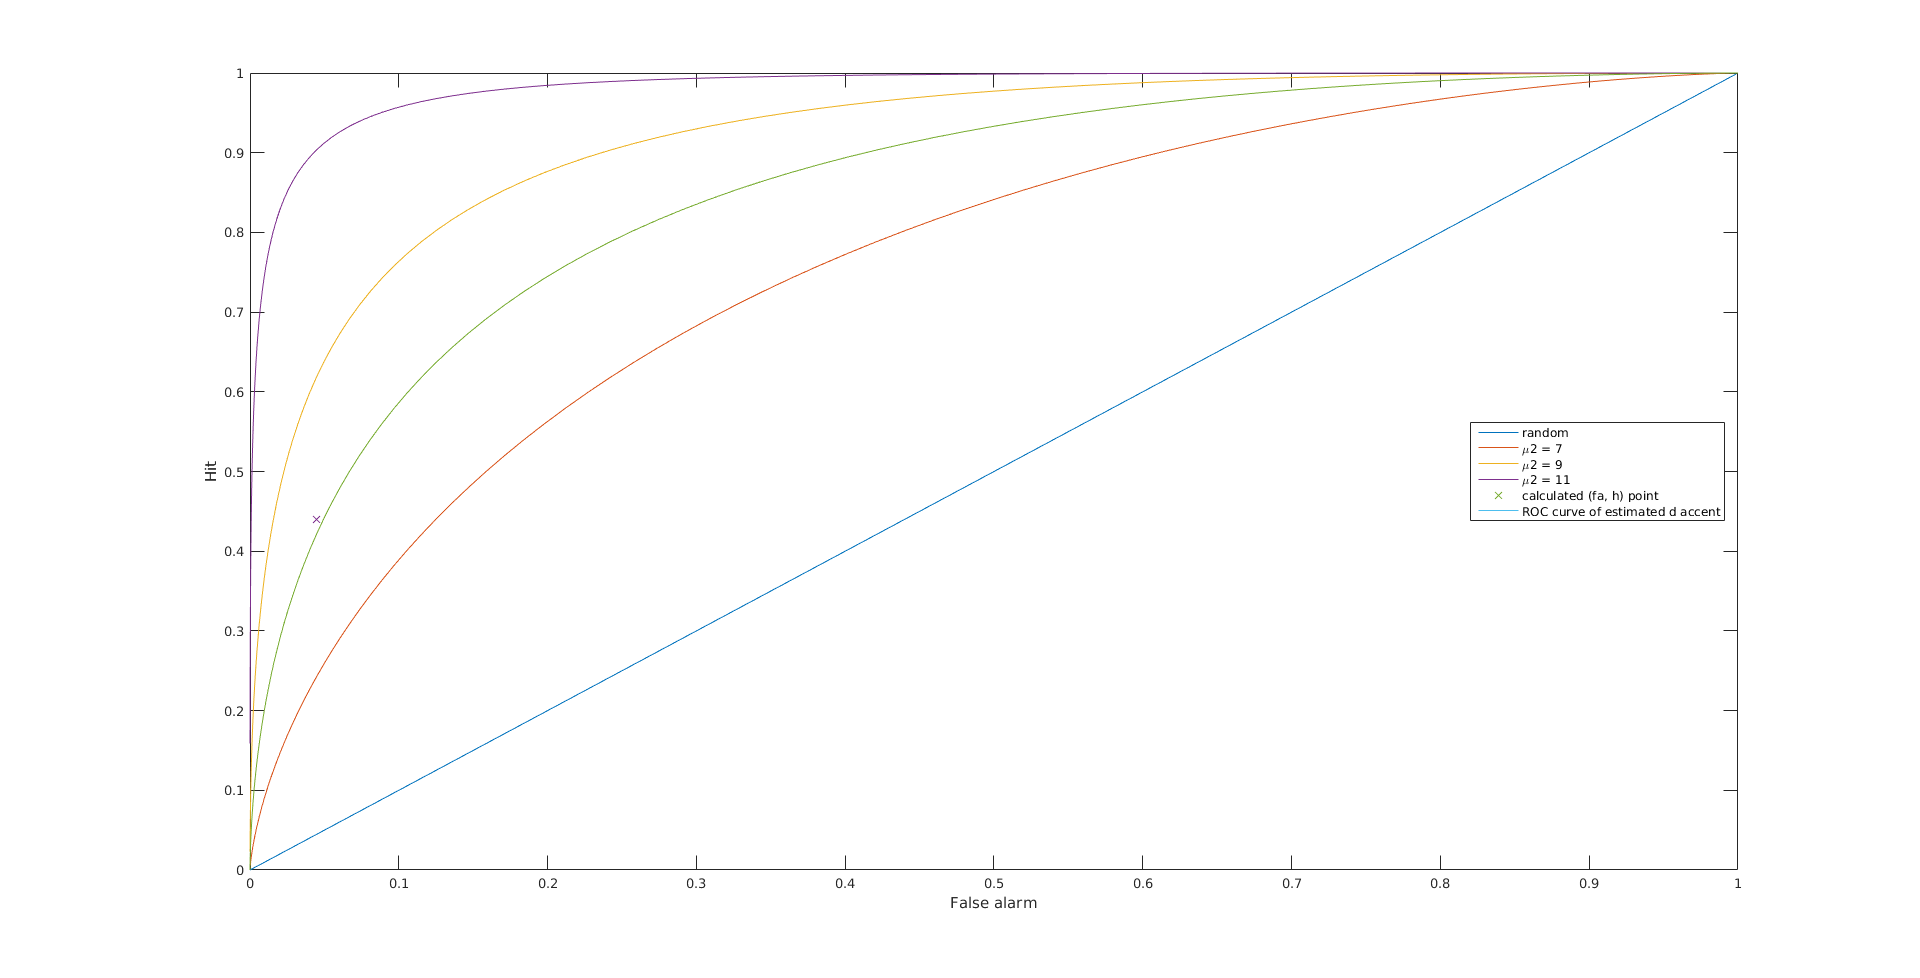
\includegraphics[width=\textwidth]{assign1_2b.png}
 \caption{Plot of the $(fa, h)$ point, the ROC-curves for $\mu_2={7, 9, 11}$, the hits $=$ false alarms marker line, and the ROC-curve with $d'=1.5$.}
 \label{fig1.2}
\end{figure}

\section{K-nearest neighbor classification}
\subsection{}
Our implementation of the KNN-function is the following:
\lstinputlisting{../Code/KNN.m}

\subsection{}
For $k={1, 3, 5, 7}$ this implementation yields the classification grid shown in figure \ref{fig2.1}:
\begin{figure}[H]
  \centering
  \begin{subfigure}{.49\textwidth}
    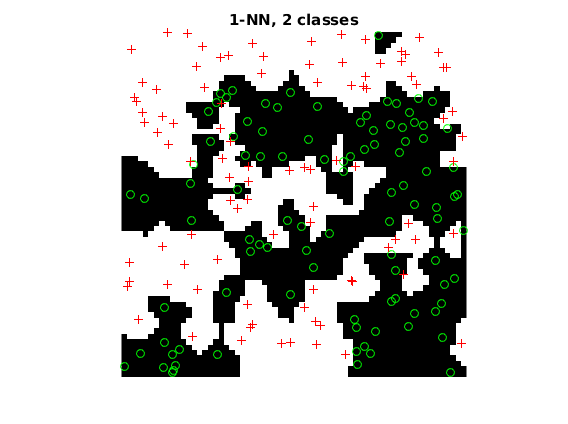
\includegraphics[width=1\linewidth]{assign2_2_1.png}
    \caption{Classification grid of the data set using KNN (for $k=1$)}
    \label{fig2.1a}
  \end{subfigure}
  \begin{subfigure}{.49\textwidth}
    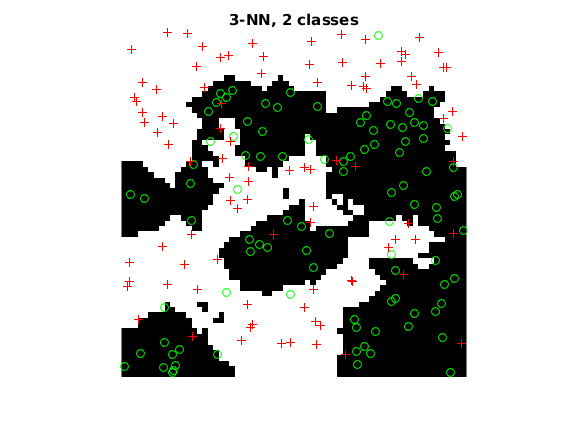
\includegraphics[width=1\linewidth]{assign2_2_3.png}
    \caption{Classification grid of the data set using KNN (for $k=3$)}
    \label{fig2.1b}
  \end{subfigure}
  \begin{subfigure}{.49\textwidth}
    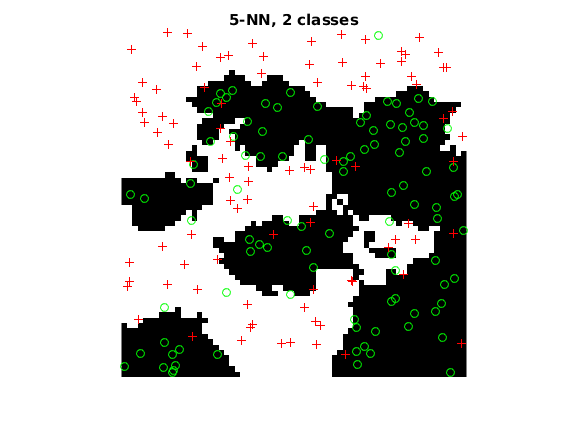
\includegraphics[width=1\textwidth]{assign2_2_5.png}
    \caption{Classification grid of the data set using KNN (for $k=5$)}
    \label{fig2.1c}
  \end{subfigure}
  \begin{subfigure}{.49\textwidth}
    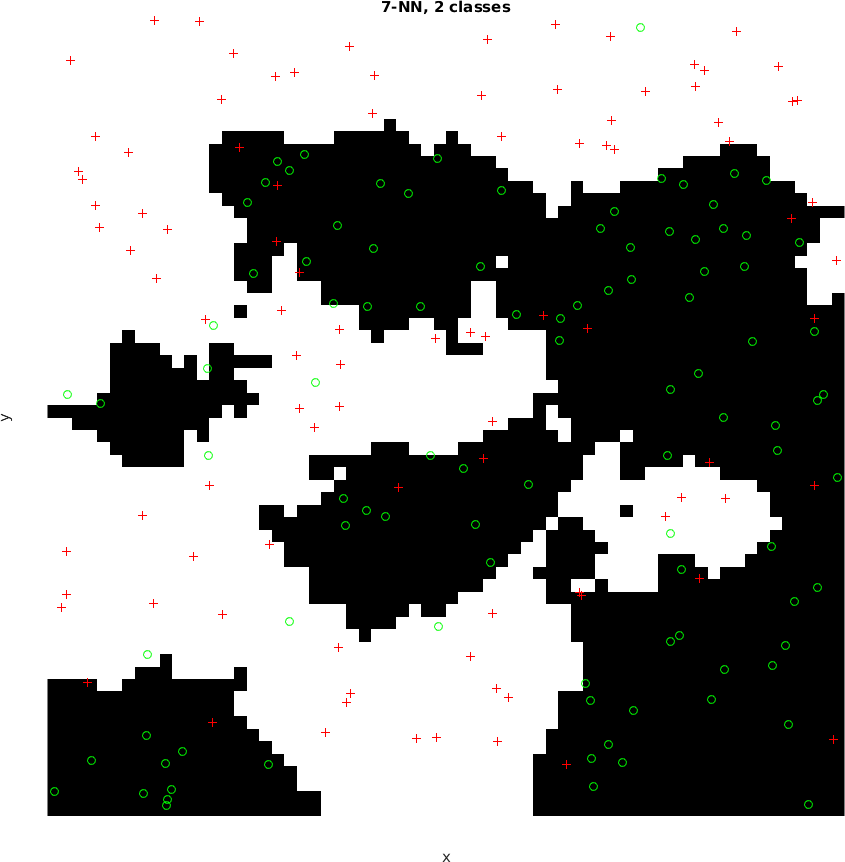
\includegraphics[width=1\textwidth]{assign2_2_7.png}
    \caption{Classification grid of the data set using KNN (for $k=7$)}
    \label{fig2.1d}
  \end{subfigure}
  \caption{Classification grids for different $k$s}
  \label{fig2.1}
\end{figure}

\subsection{}
Our implementation of the leave-one-out cross validation is given in the appendix. Figure \ref{fig2.3} gives the error rates we acquired for the diffferent values for $k$ using our implementation. The figure shows that a $k$ of 3 or 5 yields the best performance with an error rate of around 0.23. It is not illogical that the optimal $k$ is such a value. 

On the one hand a $k$ of 1 performs worse, because it does not account for outliers. With a $k$ of 1 outliers would classify a number of data points incorrectly, while increasing $k$ to 3 would already correct for that, because it is very unlikely that two outliers would be that close to each other that they would together misclassify a data point (you could even argue whether they would actually be outliers if they are close to each other). 

On the other hand when $k$ would become too high, data points are prone to be misclassified when they are closer to the decision boundary (for example when there are multiple points of the other class on the other side of the decision boundary which would be taken into account).

\begin{figure}[H]
 \centering
 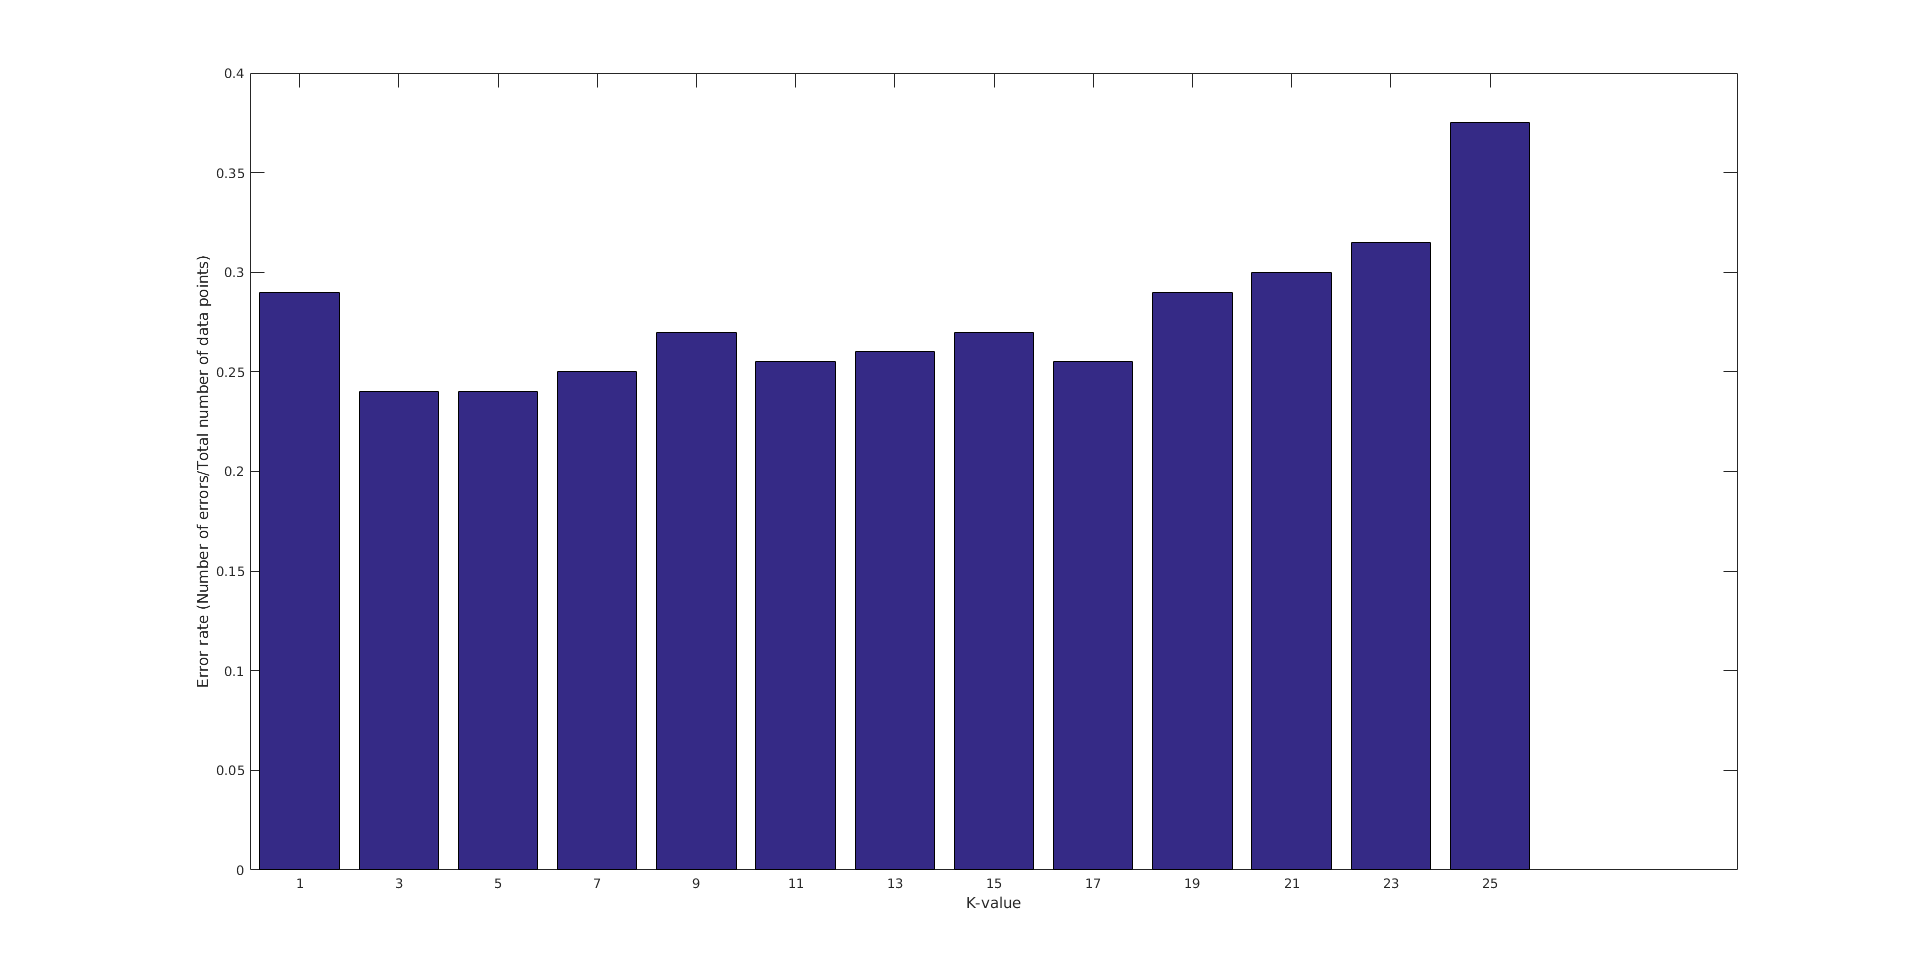
\includegraphics[width=\textwidth]{assign2_3.png}
 \caption{Error rate for different values of $k$ using leave-one-out cross validation.}
 \label{fig2.3}
\end{figure}

\subsection{}
To do classification for four classes we changed the parameter of number of classes to 4 and added the new classes to the plots. This resulted in the classification grids shown in figure \ref{fig2.4_a}. Cross validation with four classes yields the error rates given in figure \ref{fig2.4_b}. The figures show that again most of the points get classified correctly. This time we find an optimum at only a k of 5. The average error rate does seem to be higher than with two classes though. This seems logical, because with random data you would expect that with more classes there is a higher probability of a data point being classified into the wrong class. This is however, totally dependent on the data. If the actual data represent four well divided classes, the classification would of course go better when you would actually use four classes, because when you would just use two, the data might be distributed over the two classes in such a way that there is not such a clear separation boundary as with four classes. 

In normal circumstances however, the classifier data would be seperated into logical groups instead of random groups like we do now. Then a difference in classifying performance would be logically explainable, because the data would actually represent groups already.

\begin{figure}[H]
  \centering
  \begin{subfigure}{.49\textwidth}
    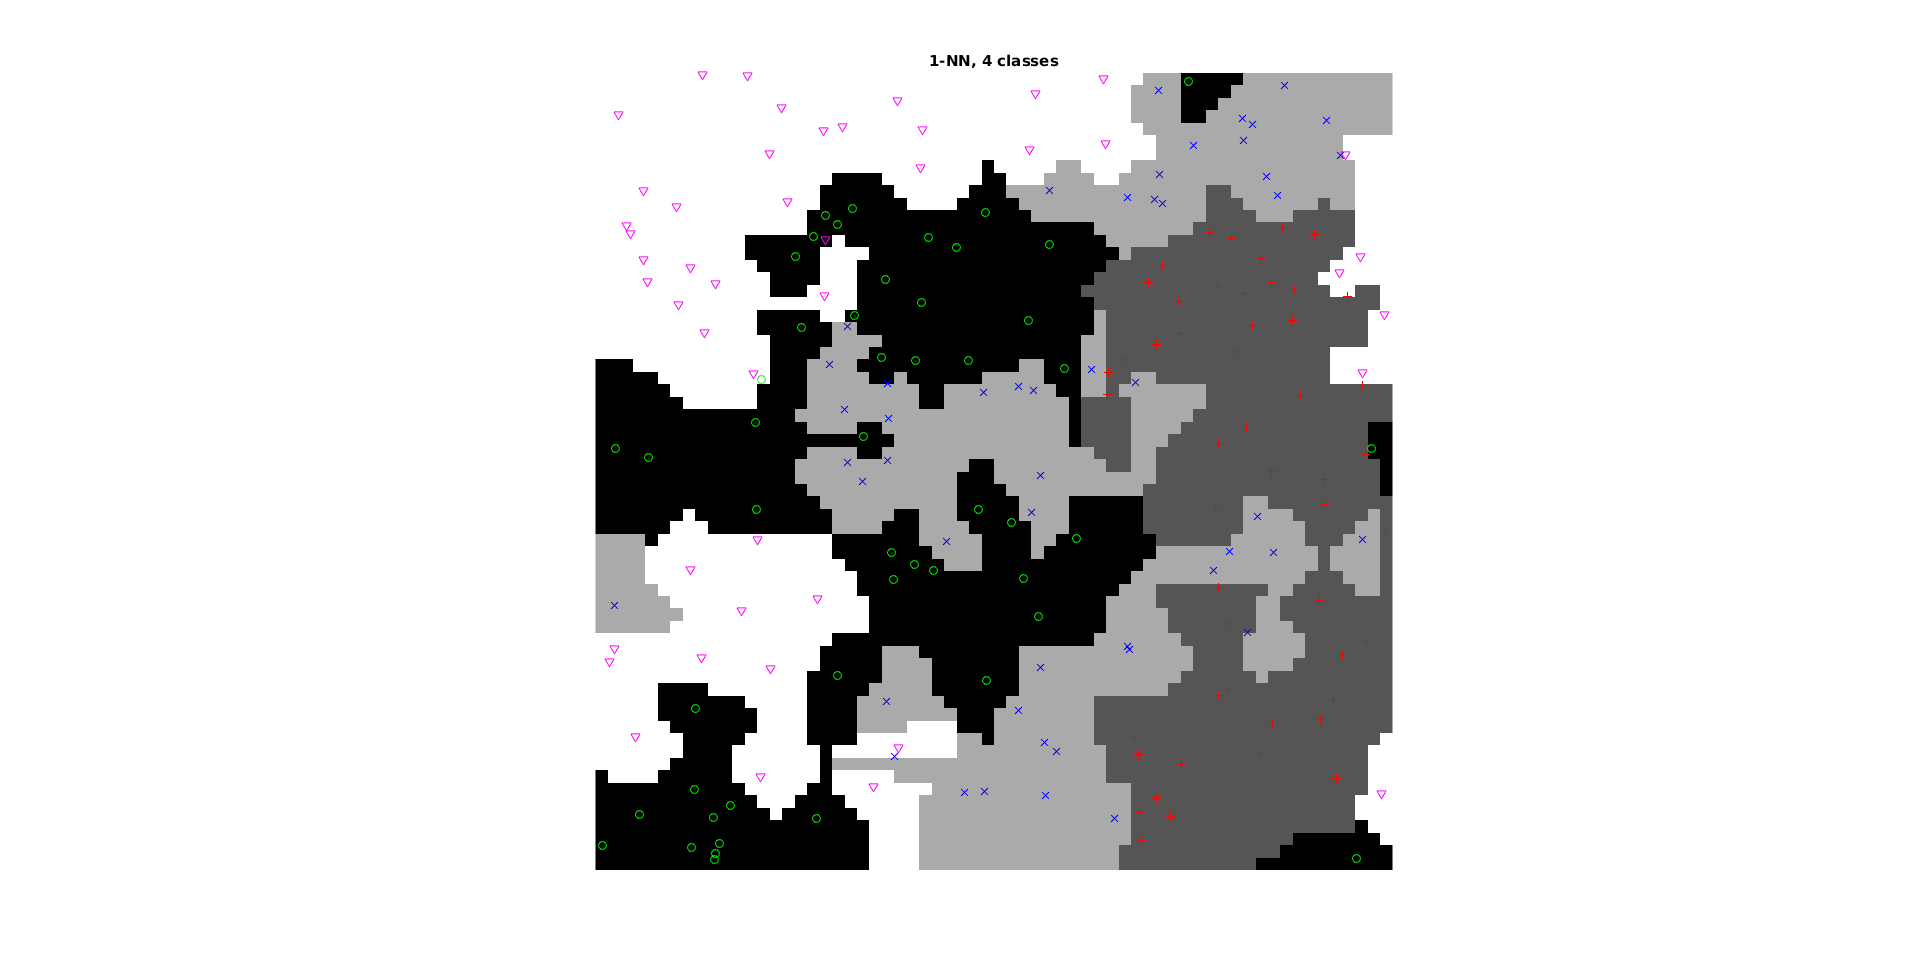
\includegraphics[width=.8\linewidth]{assign2_4_1.png}
    \caption{Classification grid of the data set using KNN (for $k=1$)}
    \label{fig2.4a}
  \end{subfigure}
  \begin{subfigure}{.49\textwidth}
    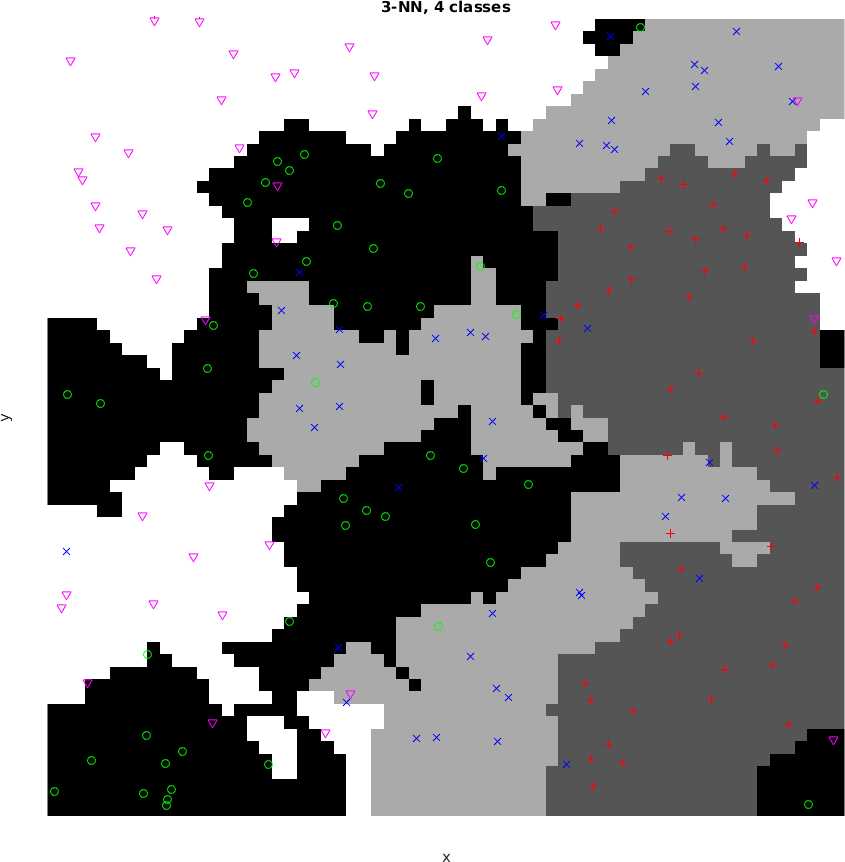
\includegraphics[width=.8\linewidth]{assign2_4_3.png}
    \caption{Classification grid of the data set using KNN (for $k=3$)}
    \label{fig2.4b}
  \end{subfigure}
  \begin{subfigure}{.49\textwidth}
    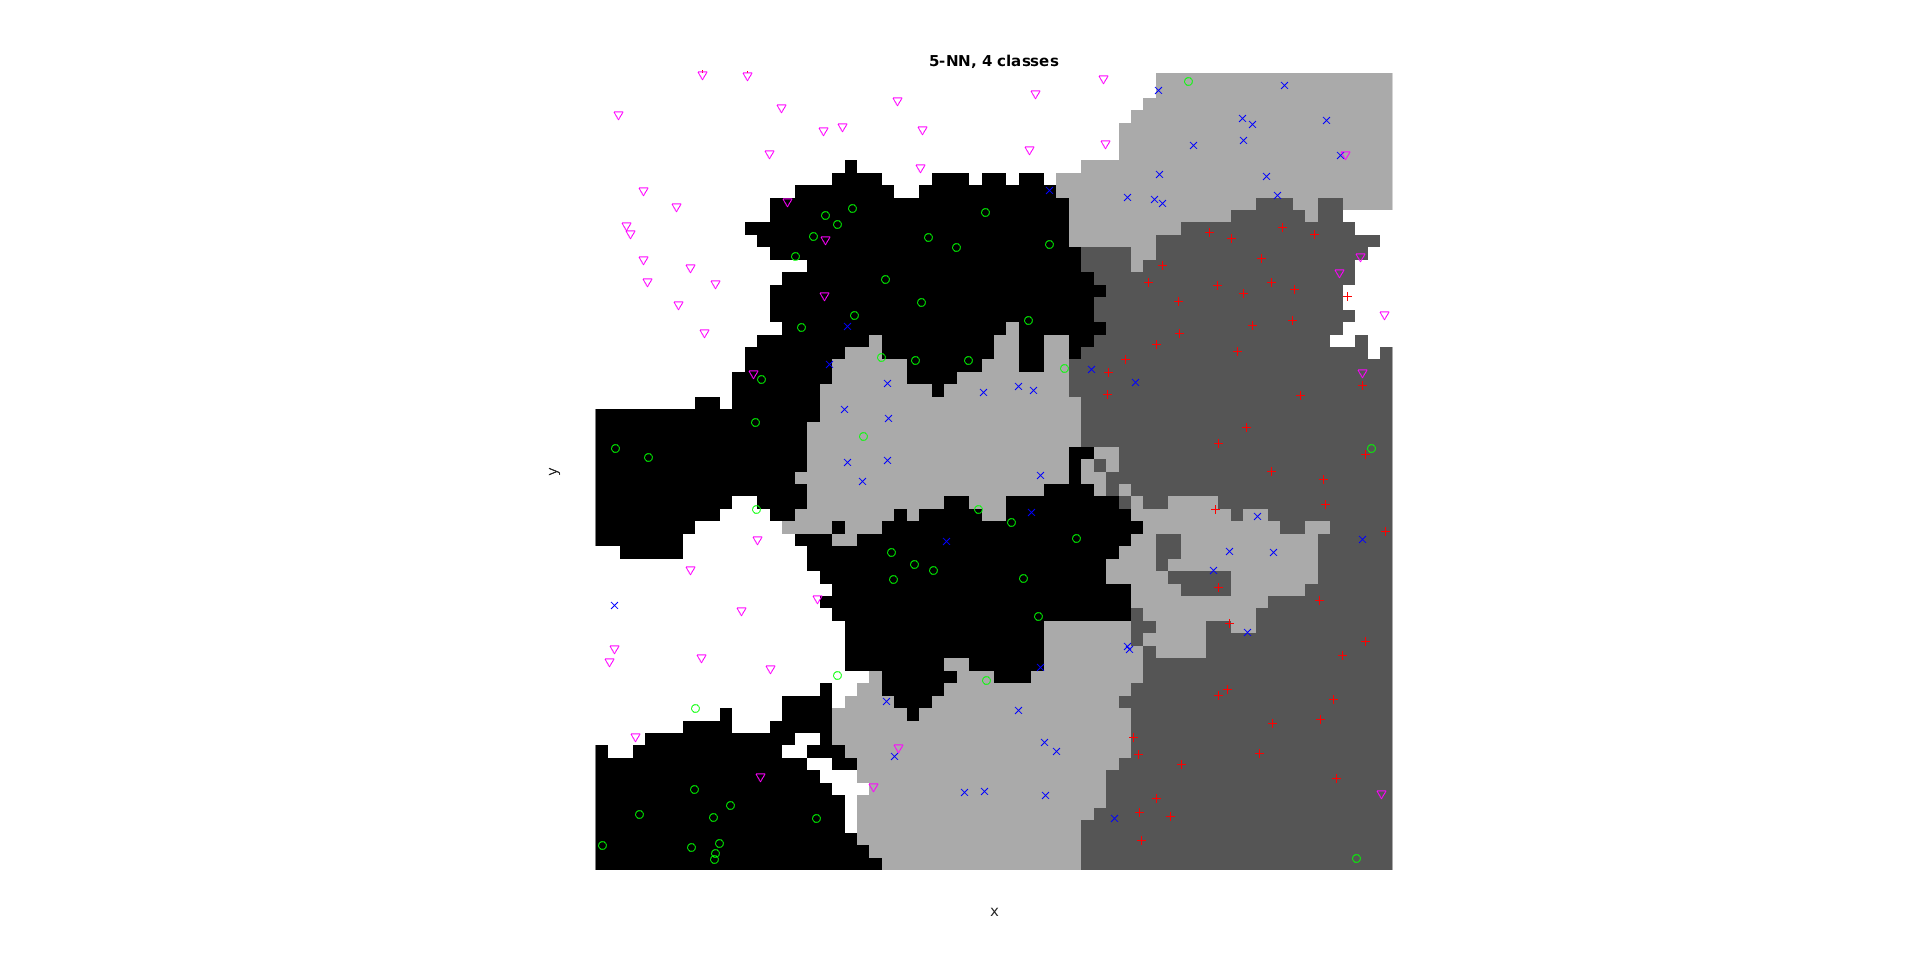
\includegraphics[width=.8\textwidth]{assign2_4_5.png}
    \caption{Classification grid of the data set using KNN (for $k=5$)}
    \label{fig2.4c}
  \end{subfigure}
  \begin{subfigure}{.49\textwidth}
    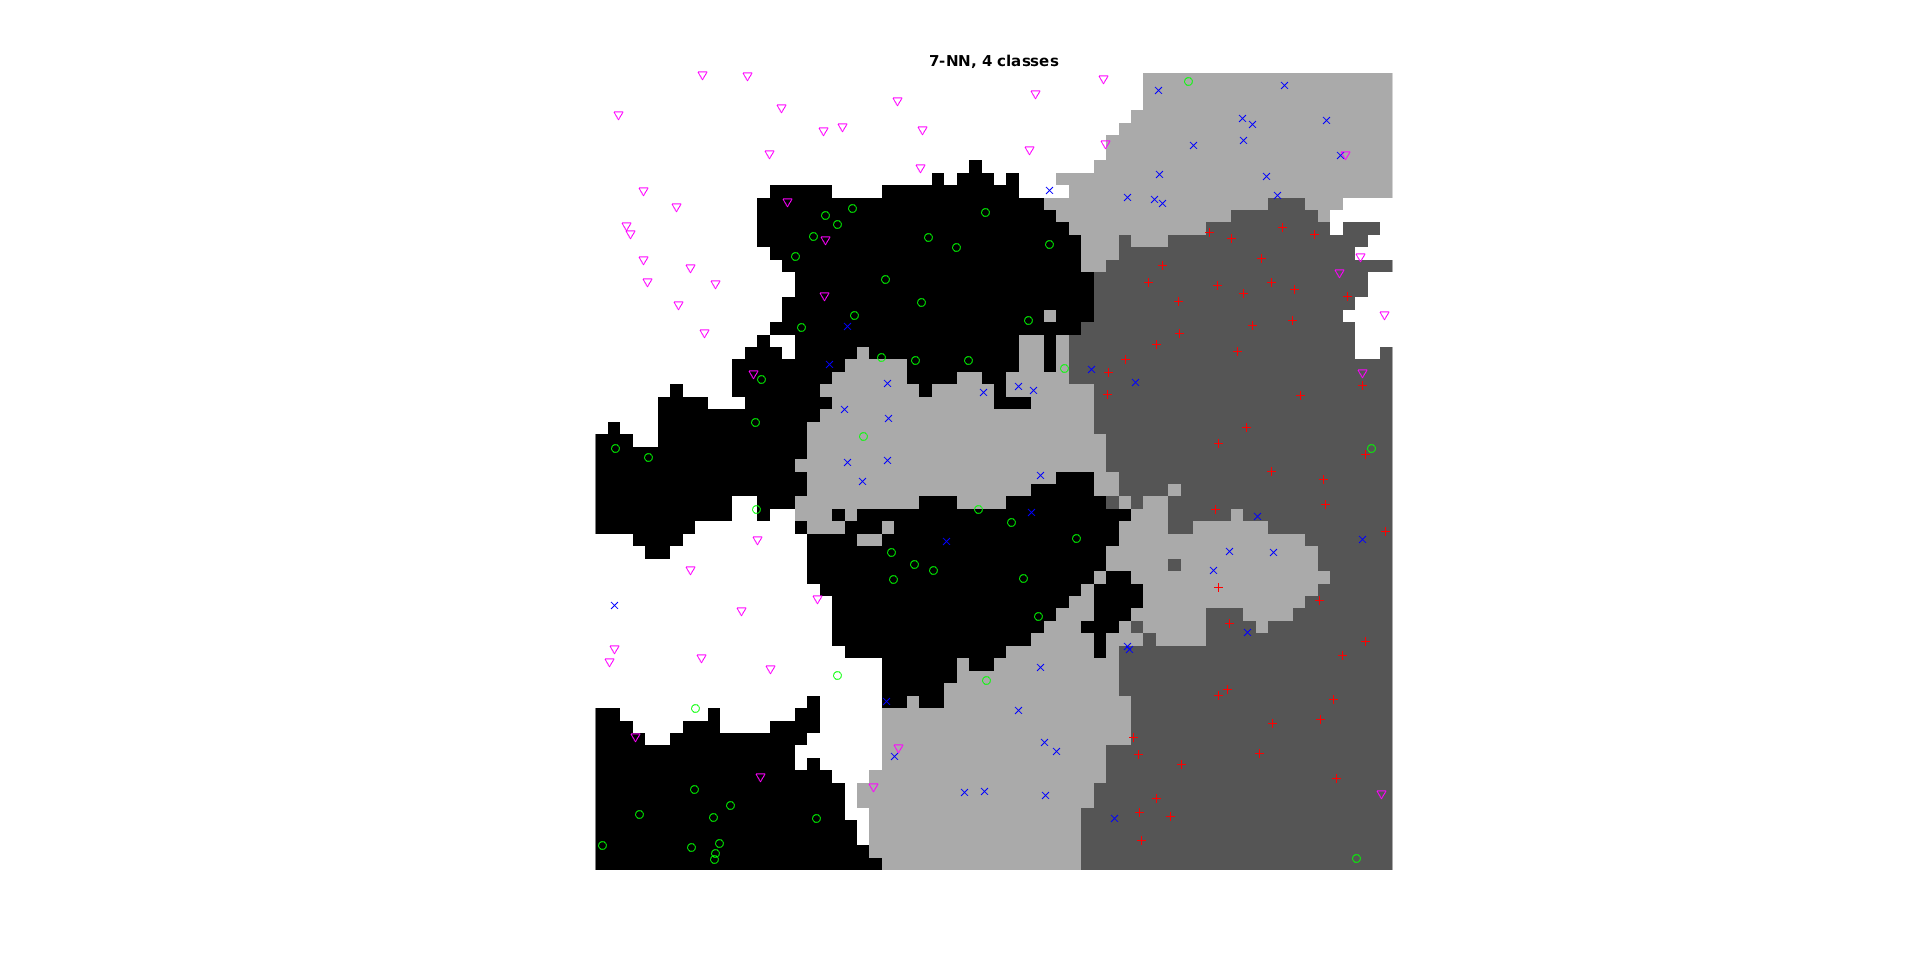
\includegraphics[width=.8\textwidth]{assign2_4_7.png}
    \caption{Classification grid of the data set using KNN (for $k=7$)}
    \label{fig2.4d}
  \end{subfigure}
  \caption{Classification grids for different $k$s}
  \label{fig2.4_a}
\end{figure}

\begin{figure}[H]
 \centering
 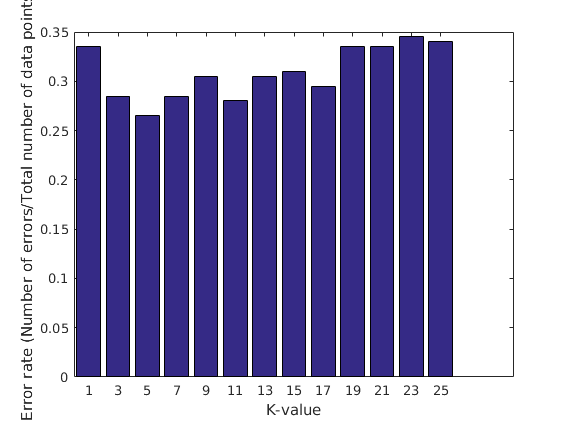
\includegraphics[width=.7\textwidth]{assign2_4_b.png}
 \caption{Error rate for different values of $k$ using leave-one-out cross validation.}
 \label{fig2.4_b}
\end{figure}

\section{Parzen windows, posterior probabilities}
\subsection{}
\autoref{tab3.1} gives the densities computed using the code given in the appendix (note that both the file assign3.m and phi.m were used):

\begin{table}[H]
 \centering
 \caption{The densities for the three points for every class ($h=1$}
 \begin{tabular}{c|c|c|c}
  Point & Class 1 & Class 2 & Class 3 \\
  \hline
  $x_1$ & $8.0e^{-3}$ & $3.0e^{-2}$ & $2.5e^{-2}$ \\
  $x_2$ & $9.7e^{-3}$ & $3.1e^{-2}$ & $1.4e^{-3}$ \\
  $x_3$ & $1.4e^{-4}$ & $6.8e^{-5}$ & $4.8e^{-6}$ \\
 \end{tabular}
 \label{tab3.1}
\end{table}

\subsection{}
The priors are 10/30 for each category, so ${P_1, P_2, P_3} = 1/3$.

\subsection{}
We used the following function to compute the posterior probabilities:
\begin{equation}
 P_n(\omega_i|x) = \frac{p_n(x,\omega_i)P(\omega_i)}{\sum_{j=1}^cp_n(x,\omega_j)P(\omega_j)}
\end{equation}

Filling in this function resulted in the posterior probabilities given in \autoref{tab3.2}.
\begin{table}[H]
 \centering
 \caption{The posterior probabilities for the three points for every class ($h=1$)}
 \begin{tabular}{c|c|c|c}
  Point & Class 1 & Class 2 & Class 3 \\
  \hline
  $x_1$ & 0.13 & 0.47 & 0.40 \\
  $x_2$ & $0.18$ & $0.56$ & $0.26$ \\
  $x_3$ & $0.65$ & $0.32$ & $0.02$ \\
 \end{tabular}
 \label{tab3.2}
\end{table}
Using \autoref{tab3.2} we classified the points as follows (the highest posterior probability determines their class):
\begin{itemize}
 \item $x_1$: class 2
 \item $x_2$: class 2
 \item $x_3$: class 1
\end{itemize}

\subsection{}
We computed the following densities using the code given in the appendix:
\begin{table}[H]
 \centering
 \caption{The posterior probabilities for the three point for every class ($h=2$)}
 \begin{tabular}{c|c|c|c}
  Point & Class 1 & Class 2 & Class 3 \\
  \hline
  $x_1$ & 0.18 & 0.42 & 0.40 \\
  $x_2$ & 0.19 & 0.45 & 0.36 \\
  $x_3$ & 0.29 & 0.49 & 0.22 \\
 \end{tabular}
 \label{tab3.3}
\end{table}
This yields the following classification:
\begin{itemize}
 \item $x_1$: class 2
 \item $x_2$: class 2
 \item $x_3$: class 2
\end{itemize}

\subsection{}
Using our implementation for KNN from assignment 2 we get the following classes for the three points (using $k=1$):
\begin{itemize}
 \item $x_1$: class 3
 \item $x_2$: class 1
 \item $x_3$: class 1
\end{itemize}



\subsection{}
Using $k=5$ our KNN-implementation yields the following classes:
\begin{itemize}
 \item $x_1$: class 3
 \item $x_2$: class 2
 \item $x_3$: class 1
\end{itemize}

The different results for the Parzen window approach and the KNN-approach yield quite different outcomes. Within both of the algorithms the results for the different parameter settings do overlap for 2 of the three points, but between the results of the algorithms we only see overlap of one point. 

This is possible because the methods both define their respective `influence regions'. In the KNN-method the amount of nearest neighbors ($k$) defines the radius of the region in which neighbors have influence on the data point that needs to be classified. So the KNN `looks' in a circle (euclidean) or diamond (Manhattan) around the data point. On the other hand the Parzen window method uses squares around the to be classified points. This means that other points could fall into the Parzen region and influence the classification of a point than by using KNN, explaining why differences in classification can occur. You would expect that these differences would become more prevalent when $h$ and $k$ become larger, because the relative difference between the two areas becomes larger as well. We do not see this from our experiment though, but of course we only compared three data points classified on the basis of a small data set.

\section*{Appendix}
\lstinputlisting{../Code/assign1_1.m}
\lstinputlisting{../Code/assign1_2.m}
\lstinputlisting{../Code/KNN.m}
\lstinputlisting{../Code/assign2_3.m}
\lstinputlisting{../Code/assign3.m}
\lstinputlisting{../Code/phi.m}

\end{document}
